\chapter{Random Variables and Their Properties}

\section{What is a Random Variable?}
\textbf{Random variables} are a tremendously useful concept in probability theory. In most situations of
science and general life we are not really interested in the actual outcome of a random experiment. Instead,
we care about particular properties of that outcome.

For starters, let us talk about the weather. 
Like most people living in the north of Europe, your choice of clothing
probably depends strongly on the weather. Let us assume that you have a thick winter jacket that you
put on when it is cold, a light soft-shell jacket that you wear when temperatures are mild and that you
simply wear a T-shirt or a sweater when it is warm. Let us also assume that the forecasting site you
consult every morning reports the temperatures up to one decimal. The question is: does it matter to you
whether it is $ 5.4 $ or $ 7.3 $ degrees centigrade outside when you make your decision about what to wear?
Most likely you are only interested in whether it is cold, mild or warm. This may obviously vary according
to your own perception of warmth and cold. Here we will assume that it is cold whenever the temperature
is below 10 degrees, mild between 10 and 20 degrees (inclusive) and warm whenever the temperature rises
above 20 degrees. So what you are really interested in, at least as far as clothing is concerned, is 
whether the temperature $ t $ is $ t < 10 $ or $ 10 \leq t \leq 20 $ or $ t > 20 $. What we are looking for
is a way of transforming outcomes from the temperature scale into judgements of perceived temperature.

Another example is the lottery. Let us again consider the German lottery where you have to correctly 
predict 6 out of 49 numbers all of which are drawn \textit{independently} 
and \textit{uniformly at random} (you should be able to understand the first term by now; after reading
this chapter, you will also understand the second). You get the main prize if you predict all these items
correctly. However, pay-outs start from three correctly predicted numbers and increase for each additional
number that you got right. So what do you really care about when playing the lottery? Does it matter to
you whether or not you correctly predicted the number 39? Probably not. All you care about is how many of
the numbers you got right.

Observe that one possible way of modelling the sample space for the lottery situation is the following:

\begin{align}
\Omega = \{(b_{1}, \ldots, b_{6}, c_{1}, \ldots, c_{6}) \mid &1 \leq b_{1} < b_2 < \ldots < b_{6} \leq 49;\\
& c_{1}, \ldots, c_{6} \in \{0,1\} \} \nonumber
\end{align}

This rather cumbersome expression states that we draw 6 balls from an urn of 49 balls without replacement (and then sort them). We also add indicators of whether we predicted each ball drawn correctly. Note that we did not model what exactly our prediction was, but only if we predicted a number correctly. So again the question arises of how we can transform outcomes from this sample space into
the events that we actually care about (namely how many balls we predicted correctly)?

\medskip
After this little motivating section, let us formally define what a random variable is.

\begin{Definition}[Real random variable]
A (real) random variable (RV) $X$ on a probability space $(\Omega, \mathcal{A}, \mathbb{P})$ is a function
$$ X: \Omega \rightarrow \mathbb{R} $$
where we require that for
all $ r \in \mathbb{R} $, the set $ A = \{\omega| X(\omega) \leq r\} $ is in the event space $ \mathcal{A}$.
\end{Definition}

Notice that the naming of the random variable is arbitrary but by convention we will often use the capital letters
$ X,Y,Z $. Also, as you can see, RVs are defined on an entire probability space. The reason is that
we want to have a probability measure associated with our sample space. 
In fact, this probability measure is the reason why we can see random variables as taking on their values
in a random way. Moreover, since we can only measure events from our event space, the condition on RVs
ensures that we can in fact measure the probability of each real value which a RV may map an outcome to.
In technical terms, we are thus making sure that the pre-image of the RV is \textit{measurable}.

Let us define a random variable for the weather situation. 
\begin{equation} \label{weatherRV}
X(t) = 
\begin{cases}
1 & t < 10 \, , \\
2 & 10 \leq t \leq 20 \, ,\\
3 & t > 2 \, .
\end{cases}
\end{equation}

In principle we can easily determine the probability of each of the values of this RV. However, we did
not bother to define a sample space and associated probability measure, mostly because we would have to
restrict the possible temperatures to those that we think are reasonable. Nevertheless, this is something
that you can do yourself.

\begin{Exercise}
Define an upper and lower bound for temperature values (make sure you can actually get all three perceived
degrees of warmth). These bounds will lead you to a discrete sample space since we postulated
that the website we consult only reports temperatures up to one decimal place after the comma. Then impose
any probability measure on the associated event space. Finally, compute the probability of each of the
values of the RV $ X $ from Equation~\eqref{weatherRV}.
\end{Exercise}

We can do the same for the lottery. Our random variable would then look as follows:
\begin{equation}\label{lotteryRV}
X(\omega) = \overset{6}{\underset{i=1}{\sum}} c_{i}
\end{equation}

Whenever a RV assumes a particular value, we write $ X=x $. Thus, if $ X $ in Equation~\eqref{lotteryRV} assumes the
value $ 4 $, i.e.\ we guessed four balls correctly, we would write $ X=4 $. And here comes the function
that computes the probability that this event happens.

\begin{Definition}[Probability distribution]
The discrete probability distribution of a RV $ X $ is denoted by
$P_X$ and is defined as the function
$$ P_X(X=x) := \mathbb{P}( \, \{\omega \mid X(\omega)=x\} \, ) $$
In the literature, often one of the two mentions of $X$ is dropped from the
notation, resulting in $P(X=x)$ or $P_X(x)$.
\end{Definition}

What is $ P(X=4) $ for the lottery example? Recall that there are 
$ a = \binom{49}{6} $ sequences of balls that we can draw (6 out of 49 balls).
In our modelling of the scenario, we also have to take
into account whether or not we correctly predicted each ball. Notice that the indicator $ c_{i} $ is a function of our predictions. 
If our prediction $ v_{1}, \ldots, v_{6} $ are ordered in ascending fashion, then
\begin{equation*}
c_{i} = 
\begin{cases}
1 & \mbox{if } v_{i} = b_{i} \\
0 & otherwise
\end{cases}
\end{equation*}

The unfairness of the lottery comes from the fact that the player has to pick out of a large number of sequences only very few of which will have more than three
numbers in common with the sequence that ends up being drawn. Let us apply this intuition to our example.
There are $ \binom{6}{4}\binom{43}{2}$ ways in which your predictions can get exactly 4 numbers right.
This is because there are $ \binom{6}{4} $ ways to guess 4 out of 6 numbers correctly and $ \binom{43}{2} $ ways to choose any two out of the 43 numbers that were not 
drawn. In total there are 
\begin{equation}
\binom{6}{4}\binom{43}{2} = 13545
\end{equation}
ways to agree on four balls with some lottery draw. This might seem like a lot. However, if we divide this by the total number of possible lottery draws, we
find that $ P(X=4) = 0.000969 $ which is very little.   

We have just seen examples where the RV takes on a specific value. We can of course also make statements
like $ X < x $ and $ X \geq x $. This is a way of expressing that a RV assumes a value above or below a certain
threshold. The way to get the probability of this event is through the cumulative distribution function.

\newpage
\begin{Definition}[Cumulative distribution function]
The \textbf{cumulative distribution function (cdf)} of a random variable $ X $ is given by
$$ F_{X}(a) := P(X \leq a) = {\underset{x \leq a}{\sum}}P(X=x) $$
\end{Definition}

The cumulative distribution function is helpful in two ways. First of all, it allows to get the probability that
$ X $ takes on a value in a certain range. Second, it has applications in sampling algorithms, some of which we might
see during the programming part of the course. A plot of the cdf of $ Z $ is given in Figure~\ref{cdfPlot}. We can recognize that it is the cdf of a discrete
distribution because it is discontinuous. If the underlying probability distribution was continuous, so would be its cdf.

\begin{figure}[t]
\center
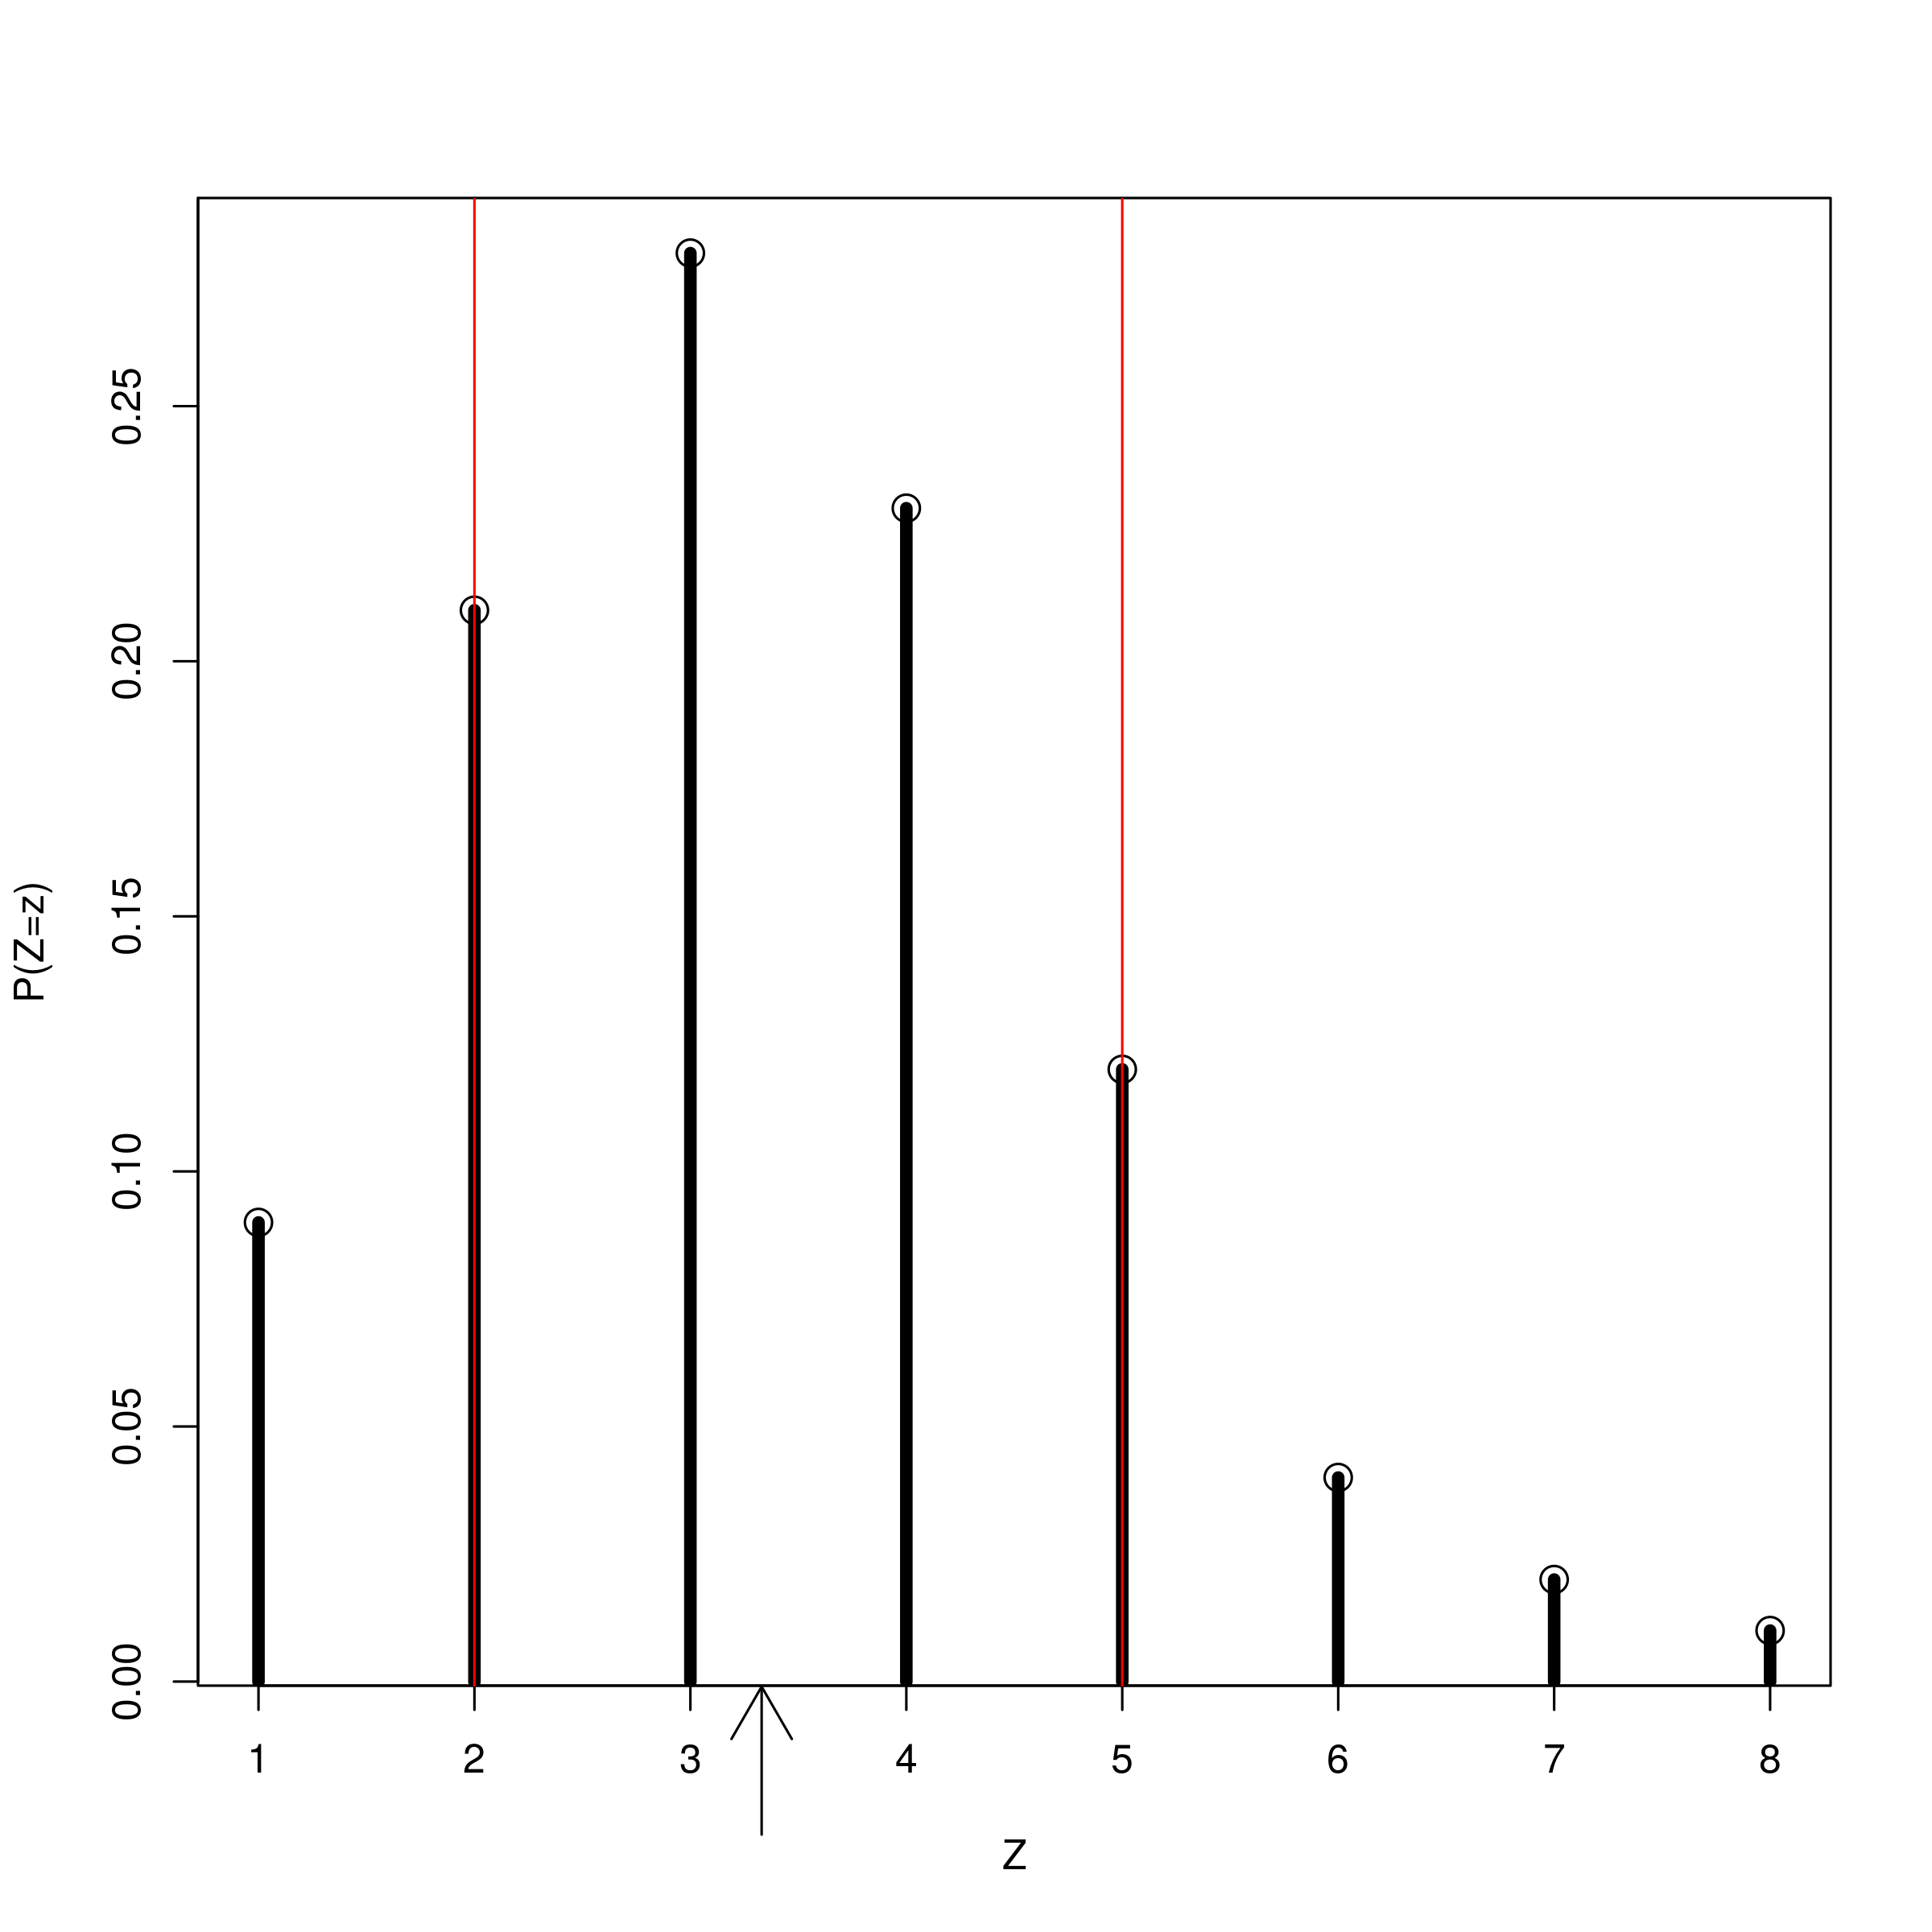
\includegraphics[scale=.4]{distribution.png}
\caption{Probability distribution of a random variable $Z$ with $ 8 $ possible values, given by $ P(Z = 1) = 0.09,  P(Z = 2) = 0.21, P(Z = 3) = 0.28, P(Z = 4) = 0.23, P(Z = 5) = 0.12, P(Z = 6) = 0.04, P(Z = 7) = 0.02$, and $ P(Z = 8) = 0.01$. The arrow indicates the expectation. This is a visualisation of 
the spike that we can plug underneath the centre of mass.}
\label{binomplot}
\end{figure}

\begin{figure}
\center
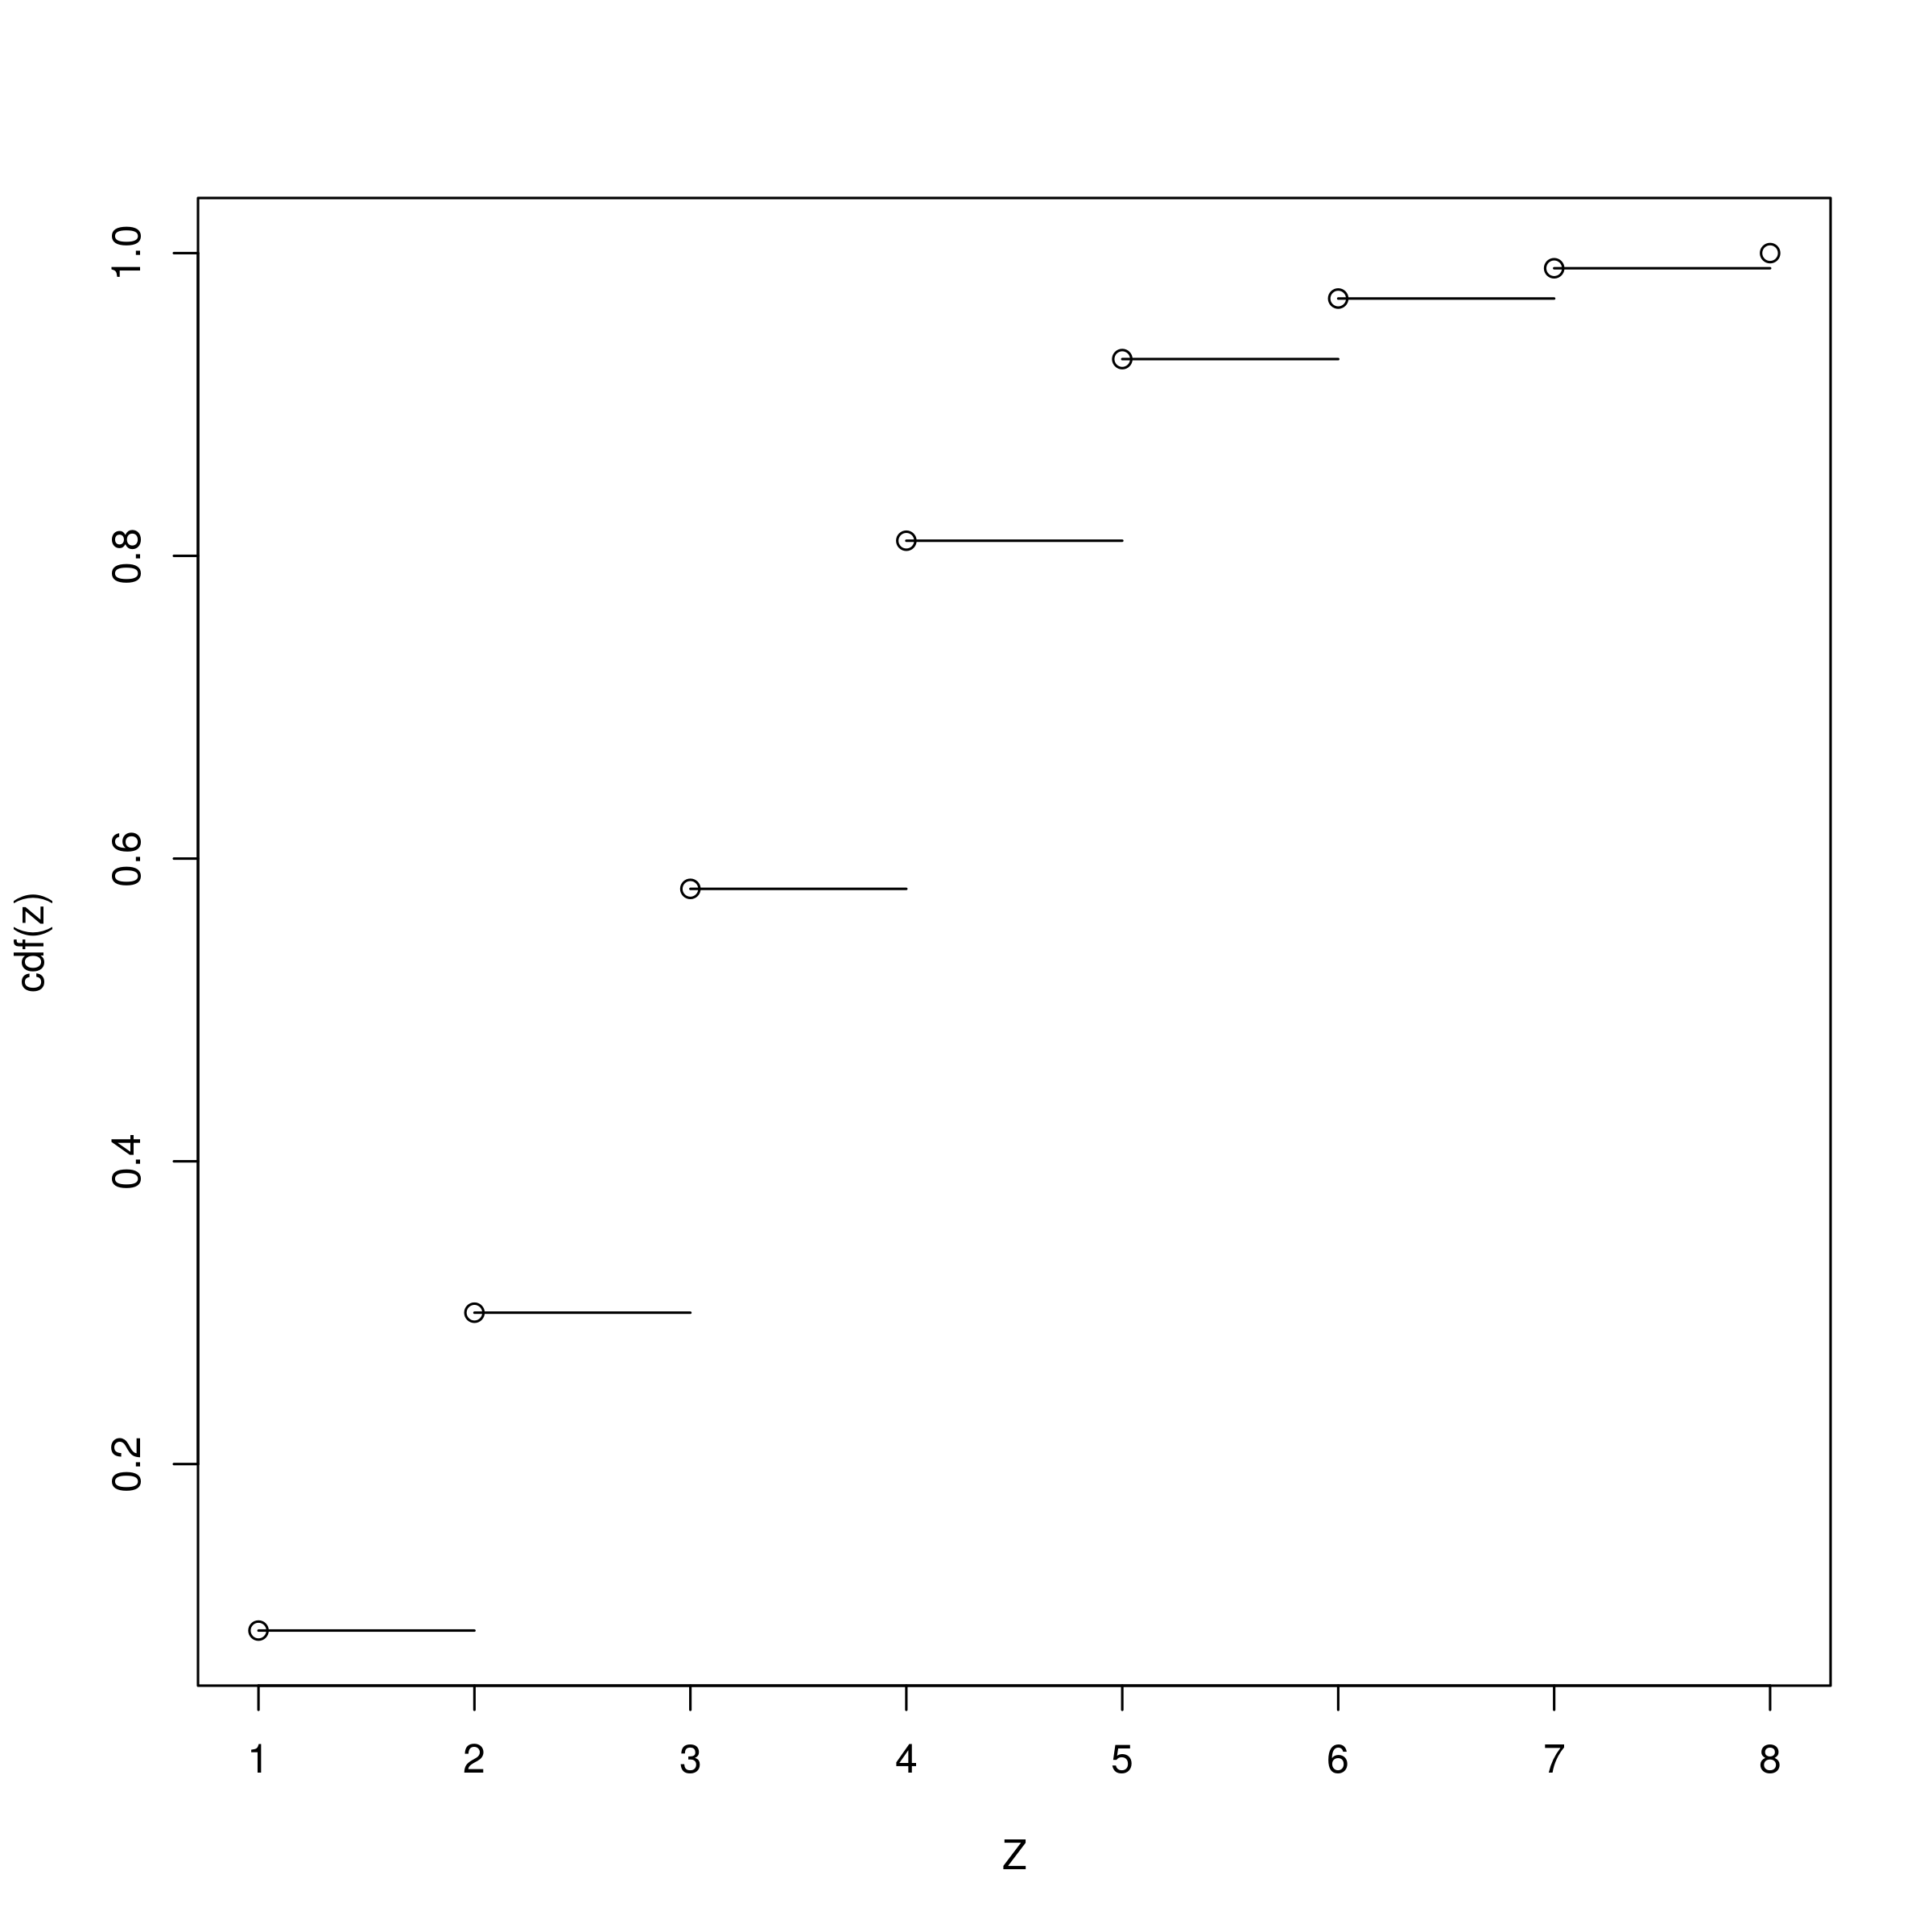
\includegraphics[scale=.4]{cdf.png}
\caption{Cumulative probability distribution of $ Z $. Observe that it stays constant in values that $ Z $ cannot take on. This cdf being discontinuous is an indicator
that the underlying probability distribution is discrete.}
\label{cdfPlot}
\end{figure}

To better understand how we can compute the probability that $ a \leq X \leq b $ for some real values $ a,b $ let us take a 
look at Figure~\ref{binomplot}. There we see a plot of the probability distribution of a random variable $ Z $. The red lines
indicate the interval that we are interested in. As a warm-up exercise, let us first compute $ P(Z \leq 2) $ and 
$ P(Z > 5) $. By looking at the plot we easily see which areas we need to consider, namely the bars to the left of 2
and to the right of 5. The height of the bars corresponds to their probability. 

We go on to compute the probability that $ Z $ is smaller or equal to 2 and that $ Z $ is bigger or equal to 5:

\begin{align}
P(Z \leq 2) =& P(Z=1) + P(Z=2) = 0.09 + 0.21 = 0.3 \\
P(Z > 5) =& P(Z=6) + P(Z=7) + P(Z=8) \\ 
=& 0.04 + 0.02 + 0.01 = 0.07 \nonumber
\end{align} 

It is straightforward to compute $ P(2 < Z \leq 5) $. If we again look at Figure~\ref{binomplot}, we see that this is
the area delimited by the red lines. Thus, $ P(Z \leq 5) $ will be an overestimate of this probability. The amount by
which it is an overestimate is exactly $ P(Z \leq 2) $. Thus we get $ P(2 < Z \leq 5) = P(Z \leq 5) - P(Z \leq 2) $.

\begin{Exercise}
We claim that you can compute $ P(2 < Z \leq 5) $ based on $ P(Z \leq 2) $ and $ P(Z > 5) $ from above. What result do
you get?
\end{Exercise}

In the case of discrete random variables, i.e.\ the ones that we are dealing with here, there is another function that is of great interest, namely the probability mass function.

\begin{Definition}[Probability mass function]
The \textbf{probability mass function (pmf)} of a random variable $ X $ is given by
$$ p(x) := P(X = x) $$
\end{Definition}

The pmf is notationally more convenient than the probability distribution but also less general. For example, the pmf does not
allow us to express that $ X $ falls in a range of values. In order to avoid confusion, we will mostly use $ X $'s 
probability distribution here. Be aware, however, that most papers that you are going to read in the future will use the pmf
instead. Regardless of whether we are using the probability distribution or the pmf, we will call the values in $ \mathbb{R} $
to which they assign positive probability, their support.

\begin{Definition}
The \textbf{support} of a random variable $ X $ is given by
$$ \supp(X) := \{x \in \mathbb{R} \mid P(X=x)>0 \} $$
\end{Definition}




\section{Expectation and Variance}

There are two major properties of probability distributions that are used to describe them. One is the center of mass, the point
at which the probability mass of the distribution is split into half. If you think of the support of $ P $ as a plank and 
of the probabilities as weights, then the center of mass is the point at which you could put an infinitely thin spike into the
plank from underneath such that the plank maintains perfect balance. In Figure~\ref{binomplot} this so-called expectation
is indicated by an arrow that can be interpreted as visualising the spike that we can plug underneath the probability plank.

\begin{Definition}[Expectation]
The \textbf{expectation} of a random variable $ X $ with respect to the distribution $ P $ is defined as
$$ \E[X] := \sum_{x \in \supp(X)} x P(X=x) \, . $$
\end{Definition}

\begin{Exercise}
Compute the expectation of the random variable $ Z $ from the previous section.
\end{Exercise}

It is important to point out that the expectation of a random variable is a real number  which does not need to in the support of $ X $. This is for example the case in Figure~\ref{binomplot} where the
expectation is fractional although all support values are integers.

The expectation comes with an interesting property that is called the \textbf{linearity of expectation}. Basically, whenever we multiply $ X $ with a constant $ a $, the expectation will also be scaled by that constant. Moreover, when we add a constant $ b $
to $ X $ the expectation will also increase/decrease by $ b $ (depending on whether $ b $ is positive or negative). Let us
prove that!

\begin{align}
\E[aX+b] &= \sum_{x \in \supp(X)} (ax+b) P(X=x) \\
&= a \!\! \sum_{x \in \supp(X)} x P(X=x) \; + \; b \!\!\!\! \sum_{x \in \supp(X)} P(X=x)\\
&= a \E(X) + b \label{sumToOne}
\end{align}

The equality in \eqref{sumToOne} follows from the fact that the sum of the probabilities of the support of a distribution is 1.
The linearity of expectation is extremely useful. Basically, if you know the expectation of a RV you also know the 
expectation of its multiples. Furthermore, by adding a constant, we basically shift each element in the support. However, this shifting
does not do anything surprising as the centre of mass shifts by the same amount.

We can actually take the expectation of any quantity, but it only has an effect on quantities that
can be cast as functions of $ X $. The expectation of a quantity that is constant with respect to $ X $ will just be that
quantity itself. More formally:
\begin{equation}
\E[b] = \sum_{x \in \supp(X)} b P(X=x) = b
\end{equation}

A class of functions of $ X $ that people are often interested in are
the moments. Moments are the powers of $ X $, so $ X $ itself is the
first moment, $ X^{2} $ is the second moment and so on. We will not
further discuss moments here, but it is useful to at least know what
they are in case you find the expression in a paper.

\medskip
After we have discussed the centre of mass, it is also interesting to look at how far the outcomes are spread around the average. Assume two random variables $ X $ and $ Y $ with
\begin{itemize}
\item $ P(X=-100) = 0.5 $; $ P(X=100) = 0.5 $
\item $ P(Y=-1000) = 0.5 $; $ P(Y=1000) = 0.5 $
\end{itemize}
The spread of $ Y $ is obviously going to be greater, although both have the same expectation. The quantity usually used to assess
the spread of a RV is the variance.

\begin{Definition}[Variance]
The variance of a RV $ X $ is given by
$$ \var(X) := \E[\, (X - \E[X])^{2} \, ] \, .$$
\end{Definition}

The expression for $ \var(X) $ is rather scary-looking but let us try to make sense of it. The inner part is the difference between
each value of the random variable and the expectation. Thus the outer expectation is just a weighted sum of differences between 
values in the support and the expectation. However, since values of $ X $ can be smaller or greater than the expectation, this
sum will be 0. Therefore we square it, leaving us with only positive values. In summary, the variance is the expectation
of the squared differences between the expectation and the values in the support of $ X $.

Computing the variance as an expectation can be cumbersome. We show how it can be done more efficiently.
\begin{align}
\var(X) &= \E[\, (X - \E[X])^{2} \, ] \\
&= \sum_{x \in \supp(X)} P(X=x) (x - \E[X])^{2} \\
&= \sum_{x \in \supp(X)} P(X=x) (x^2 - 2x\E[X] + \E[X]^{2}) \\
&= \sum_{x \in \supp(X)} P(X=x)  x^{2} -  \!\!\!\!\! \sum_{x \in \supp(X)} \!\!\!\!\! P(X=x) 2x\E[X] + \E[X]^{2} \\
&= \E[X^{2}] -   2 \E[X]^{2} + \E[X]^{2}  \\
&= \E[X^{2}] - \E[X]^{2} \, . \label{variance}
\end{align}

For most intents and purposes we will use \eqref{variance} to compute the variance. 

% Also, from here on, we will generally drop the 
% subscript indicating the distribution of the the expectation in order to save ourselves some writing.

\begin{Exercise}
Compute the variance of the RV Z from the previous section.
\end{Exercise}

Although variance is not linear, we can still try to figure out what happens when we multiply a RV by a constant or add a constant to it.
\begin{align}
\var(aX+b) &= \E[ (aX+b - \E[aX+b])^2 ] \\
&=\E[ (aX+b - a\E[X] - b)^2 ] \\
&=\E[ a^2 (X-\E[X])^2 ] \\
&= a^2 \var(X)
\end{align}

\begin{Exercise}
Give an alternative proof of $\var(aX+b) = a^2 \var(X)$ by using $\var(X)
= \E[X^{2}] - \E[X]^{2}$.
\end{Exercise}
% \begin{align}
% \E[(aX+b)^{2}] - (\E[aX+b])^{2} \\
% &= \E[(aX+b)^{2}] - (a\E[X]+b)^{2} \\
% &= \E[a^{2}X^{2} + 2abX + b^{2}] - a^{2}\E[X]^{2} - 2ab\E[X] - b^{2} \\
% &= a^{2}\E[X^{2}] + 2ab\E[X] + b^{2} - a^{2}\E[X]^{2} - 2ab\E[X] - b^{2} \\
% &= a^{2}\E[X^{2}] - a^{2}\E[X]^{2} = a^{2}\var(X) \
% \end{align}

What we see that the variance is not affected by adding a constant to the RV. This makes sense, as constant additions just shift
the expectation. However, the relation of each individual value to the expectation is not affected by that operation. On the other hand,
when we multiply each value of the RV by a constant, the variance is scaled by the square of that constant. Again, this is not surprising.
Remember that we used squaring in our definition of the variance to turn all distances from the expectation into positive numbers.
If we multiply an RV by a constant $ a $, its spread will increase in both directions by a factor of $ a $. 
Since we again want only positive differences,
we better square that increased spread. This intuitively justifies the above equalities.

\begin{figure}
\center
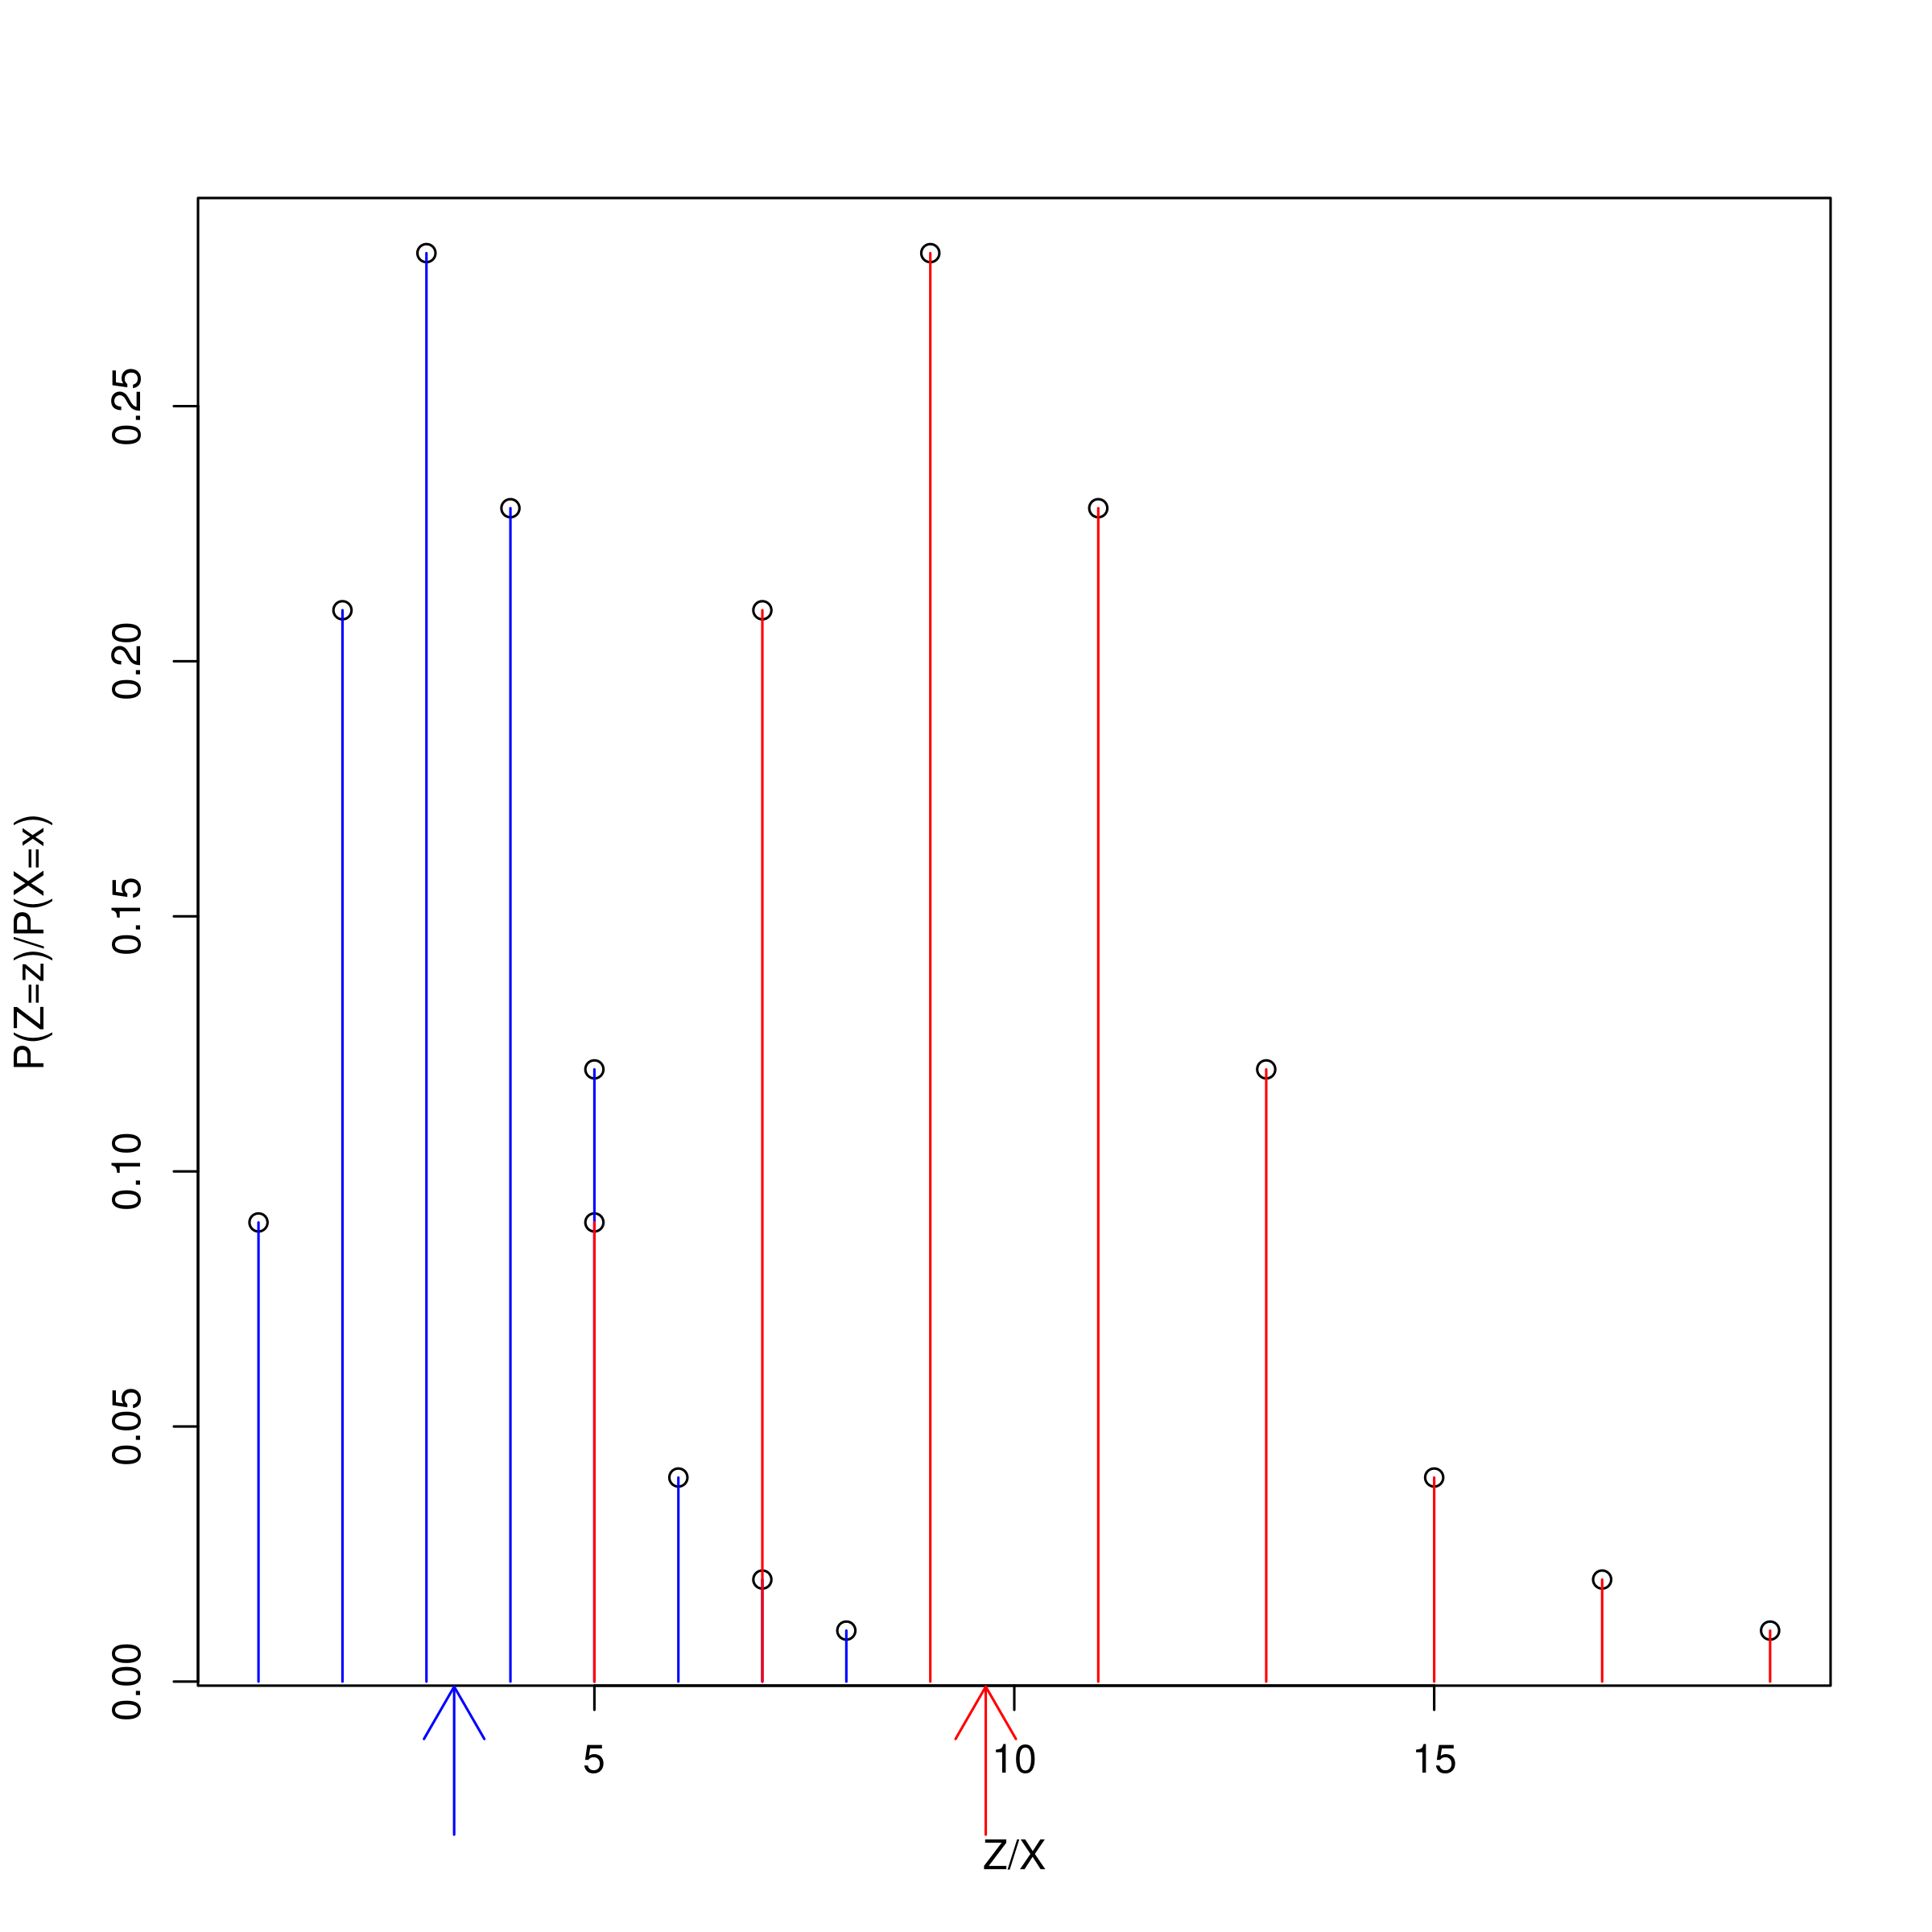
\includegraphics[scale=.4]{scaledRV.png}
\caption{Plot of RVs $ Z $ and $ X = 2Z+3 $. The arrows indicate the expectation of each distribution.}
\label{scaledRV}
\end{figure}

To gain a visual understanding of what happens when a RV gets scaled and a constant gets added to it, take a look at Figure~\ref{scaledRV}. The random variable 
$ Z $ is the same as in Figure~\ref{binomplot} and its probability distribution is plotted in blue. Figure~\ref{scaledRV} also shows the probability distribution
of another RV $ X = 2Z + 3 $ in red. As predicted by our calculations above, the expectation (indicated by the red arrow) shifts by two times its original value plus
three. Furthermore, note that the addition of three does not have any influence on the variance of $ X $. The relative distance between the elements in the support
of $ X $ is the same as the relative distance between the elements in the support of $ Z $. However, the distance between the smallest and largest value in the support
has doubled, hence increasing the variance by a factor of $ 2^{2} = 4 $.


\section{Joint and conditional distributions} \label{sec:jointconditionaldistributions}

Up to now, we have only looked at cases that could be treated with one random variable. Most interesting problems involve several RVs, however. We introduce the concept of jointly distributed random variables. What this means is that
there is a distribution over tuples of values, each from a different RV.

\begin{Definition}[Joint probability distribution]
Random variables $ X_{1}, \ldots, X_{n} $ (\textbf{abbreviated as $ X^{n}_{1} $}) 
are said to be \textbf{jointly distributed} with probability distribution $ P_{X_{1}^{n}} $ if
$$ P(X_{1}=x_{1}, \ldots, X_{n}=x_{n}) = \mathbb{P}(\, \{\omega \mid
X_{1}(\omega) = x_{1}, \ldots, X_{n}(\omega)=x_{n}\}\, ) \, . $$ 
\end{Definition}

From the above definition, we see that the random variables need to
share an underlying sample space. This also gives us more insight into
the real power of RVs: in applications, we usually do not care at all
about the underlying sample space but only about quantities
captured by the RVs. Therefore, we define a probability distribution over the
random variables of interest. Since by definition the distribution has
to fulfil conditions that allow us to interpret the distribution
as a probability measure on a probability space, we can use the distribution without worrying
about the underlying sample space.

Joint distributions are of particular interest because they make it possible to recover the probability distribution of each individual
RV as well as of smaller joint distributions. The process by which this recovery can be accomplished is known as \textbf{marginalization}. Say
we are given a joint distribution $ P_{XY} $. How can we determine the probability that $ X=x $? Our sample space is carved
up by the values that $ X $ and $ Y $ can take on. We are interested in the probability of the subset $ E = \{\omega|X(\omega)=x\} $.
Assuming that $ Y $ can take on $ n $ values $y_1,y_2,\ldots,y_n$, let us define $ F_{i} = \{\omega| Y(\omega) = y_{i}\} $ for $ 1 \leq i \leq n $.
Some (possibly all) of the $ F_{i} $ will overlap with $ E $. Thus we can partition $ E $ into $ E\cap F_{1}, \ldots, E \cap F_{n} $.
By countable additivity, we simply need to sum up the probabilities of these intersections. Observe that those probabilities correspond exactly to $ P(X=x,Y=y_{1}), \ldots, P(X=x,Y=y_{1}) $. Hence, we get to the following equality:

\begin{equation} \label{simpleMarginal}
P(X=x) = \overset{n}{\underset{i=1}{\sum}} P(X=x,Y=y_{i}) 
\end{equation}

If we set $ X = (Z_{1}, \ldots, Z_{m}) $, we can recover $ P_{Z_{1}^{m}} $ from $ P_{Z_{1}^{m}Y} $ in the same way. Likewise,
if we set $ Y = (Z_{1}, \ldots, Z_{m}) $ we get the generalization of \eqref{simpleMarginal}. We will assume that each $ Z_{j} $
can assume $ n_{j} $ values.

\begin{align}
P(X=x) = \overset{n_{1}}{\underset{j_{1}=1}{\sum}}\ldots \overset{n_{m}}{\underset{j_{m}=1}{\sum}} 
P(X=x,Z_{1}=z_{j_{1}}, \ldots, Z_{m}=z_{j_{m}})
\end{align}

For exercise purposes, it often helps to draw a joint probability table and do marginalization from there.

\begin{table}
\center
\begin{tabular}{|c|c|c|c|}
\hline
$X\backslash Y$	& 1		& 2		& 3		\\
\hline
1				& 0.15	& 0.08	& 0.07	\\
2				& 0.01	& 0.2	& 0.03	\\	
3				& 0.28	& 0.17	& 0.09	\\
\hline
\end{tabular}
\caption{Joint probability table for $ X $ and $ Y $.}
\label{jointTable}
\end{table}

\begin{Exercise}
Find the marginal distributions $ P_X $ and $ P_{Y} $ in Table~\ref{jointTable}.
\end{Exercise}

We have already seen how the joint probability of random variables links back the the probability space that underlies them.
This link makes it easy to import certain concepts that we have
gotten to know in previous chapters. In particular, we can define \textbf{conditional probability distributions}.

\begin{Definition}[Conditional probability distribution]
Let $X,Y$ be random variables with joint distribution $P_{XY}$. Let
$y$ be such that $P(Y=y)>0$. The probability of $ X = x $ conditioned on $ Y=y $ is given by
$$ P(X=x|Y=y) := \dfrac{P(X=x, Y=y)}{P(Y=y)} \, . $$
The conditional distribution of $X$ given $Y=y$ is denoted by $P_{X|Y=y}$.
\end{Definition} 

\begin{Exercise}
Compute the conditional probability distributions $ P_{X|Y=2} $ and $ P_{Y|X=1} $ from Table~\ref{jointTable}.
\end{Exercise}

Likewise, the concept of independence carries over to distributions.

\begin{Definition}[Independence of random variables]
Two random variables $ X,Y $ are independent (denoted by $ X \bot Y $)
if $P_{XY} = P_X P_Y$, i.e.\ $\forall x \in \supp(X), \forall y \in \supp(Y): P(X=x, Y=y) = P(X=x)P(Y=y) $.
\end{Definition}

As with events, independence is equivalent to stating that $ P_{X|Y} = P_{X} $ (and
to $P_{Y|X}=P_Y$). Moreover, independence makes it much easier to calculate the expectation and variance of functions of jointly distributed random variables.
%\footnote{Notice that the joint random variable $(X,Y)$ is not a \emph{real-valued} random variable anymore. Hence $\E[X,Y]$ and $\var(X,Y$) are not defined. Rather, we can define a new (real-valued) random variable as $f(X,Y)$ for a function $f: \mathbb{R} \times \mathbb{R} \rightarrow \mathbb{R}$. and compute $\E[f(X,Y)]$ and $\var(f(X,Y))$.} 
For independent $X$ and $Y$, we have
\begin{align}
\E[XY] &= \sum_{x \in \supp(X)} \sum_{y \in \supp(Y)} P(X=x,Y=y) x y \\
&= \sum_{x \in \supp(X)} \sum_{y \in \supp(Y)} P(X=x)P(Y=y) x y \\
&= \sum_{x \in \supp(X)} P(X=x)x \sum_{y \in \supp(Y)}  P(Y=y) y \\
&= \E[X]\E[Y]
\end{align}

Similarly, it does not really make sense to talk about the variance of two random variables (at least not as one single
value). However, we can again compute the variance of functions. For addition, independence again makes our lives
much easier.

\begin{Exercise}
Show that for independent RVs $X$ and $Y$, we have that $ \var(X + Y) =
\var(X) + \var(Y) $. Give an example of dependent $X$ and $Y$ with $ \var(X + Y) \neq
\var(X) + \var(Y) $.
\end{Exercise}


While the variance of two jointly distributed variables is not defined, there is the concept of \textbf{covariance}. The variance measures the spread
of one RV, the covariance measures to what extend two variables spread together. In other words, to what extend two variables change together systematically. 
\begin{Definition}[Covariance]
The covariance of two RVs $ X,Y $ with joint distribution $P_{XY}$ is defined by
$$ cov(X,Y) := \E\left[\left(X - \E[X]\right)\left(Y - E[Y]\right)\right] $$
\end{Definition}

\begin{Exercise}
Define any two random variables with joint distribution $ P_{XY} $ such that $ cov(X,Y) < 0 $.
\end{Exercise}

Notice that covariance is symmetric. Let us for a moment look at it as a function of $ X $ only. Then, for every value $ y \in \supp{Y} $, the quantity 
$ (y - \E[Y]) = c_{y} \in \mathbb{R} $
serves as a coefficient which scales $ (X - E[X]) $ and that thus determines how much the covariance changes as we change $ P_{X} $. 
Under this view, the covariance is be a linear function
of $ X $. The precise meaning of saying that the covariance measures the systematic joint change of $ X $ and $ Y $ is thus that it measures their linear dependence
on each other.

Another interesting question is to what extend two variables influence each other relatively, i.e.\ how much the outcome of one
determines the outcome of the other. The general concept behind this question is called \textbf{correlation}. Correlation is always a measure of dependence
between two RVs. Recall that the definition of independence is binary -- either two variables are independent or they are not.
Correlation allows us to make more fine-grained relationships between RVs. There are different measures of correlation.
We present the quasi-standard one here.
\begin{Definition}[Pearson Correlation]
The Pearson correlation coefficient between to RVs $ X $ and $ Y $ with finite non-zero variance and joint distribution $P_{XY}$ is given as
$$ \rho_{XY} = \frac{cov(X,Y)}{\sigma(X)\sigma(Y)} $$
where $ \sigma(X) = \sqrt{\var(X)} $.
\end{Definition}


The correlation coefficient $ \rho $ measure the dependence between variables through their (co)variances. It does so by normalizing each of the two RVs to having
unit variance. The Pearson correlation is then simply the covariance of the normalized variables. 
Notice that because the covariance can take on both positive and negative values, the
Pearson correlation lies in the interval $ [-1,1] $. The interpretation of $ \rho_{XY} $ is thus that it measure the relative linear influence (dependence) of the 
variables on one another. This is different from the covariance which measures the absolute linear dependence that the variables have on each other. Notice that covariance 
and correlation are closely related, so much in fact that one sometimes sees the following definition of covariance.
\begin{equation}
cov(X,Y) =  \rho_{XY} \sigma(X)\sigma(Y)
\end{equation}

As with expectation and variance, independence of two variables also has consequences for their correlation and covariance.
\begin{Exercise}
Assume two RVs $ X $ and $ Y $. Show that if $ X \bot Y $ we have $ cov(X,Y) = 0 $ and $ \rho_{XY} = 0 $.
\end{Exercise}

\section{Some Important Distributions} \label{sec:importantdistributions}

We will finish this chapter by introducing some extremely useful discrete distributions. They are very often used in
computer science to model the probability of bit strings and in linguistics and natural language processing to model
the probability of sentences. 

To get us started, let us consider coin tosses. When you toss a fair coin, the probability that it lands on heads is 0.5 and
so is the probability that it lands on tails. Let $ 1 $ stand for heads and $ 0 $ for tails in a random variable $ X $ 
modelling coin tosses. We can formalize this distribution as
\begin{equation*}
P(X=x) = 0.5^{x}\times 0.5^{1-x} = 0.5 \mbox{ for $x \in \{0,1\}$ .}
\end{equation*}

Notice though that not all coins are fair and that in general we want to allow for probabilities that are not equal. 
We will therefore introduce a parameter $ \theta $ that regulates the probability that we observe heads. In the
above equation, we set $ \theta = 0.5 $. What happens if we set $ \theta = 0.3 $?
\begin{equation}
P(X=x) = 0.3^{x} \times 0.7^{1-x} = 
\begin{cases}
0.3 & \mbox{ if $x=1$} \, , \\
0.7 & \mbox{ if $x=0$} \, .
\end{cases}
\end{equation}

Where did we get the 0.7 from? Well, we know that the coin has to land on either heads or tails. Thus, if the probability
to land on heads is $ 0.3 $ the probability to land on tails has to be $ 0.7 $. Moreover, we chose $ 1 $ as a stand-in for
landing on heads. As we would expect, $ X = 1 $ will return the $ 0.3 $ probability and $ X = 0 $ will return the probability of $ 0.7 $.

This leads to a general formulation where we do not specify the parameter $ \theta $ but leave it to be filled in. 
The resulting distribution, known as \textbf{Bernoulli distribution} (with parameter $ \theta $), is shown in Equation~\eqref{Bernoulli}.
\begin{equation}\label{Bernoulli}
P(X=x) = \theta^{x} \times (1 - \theta)^{1-x} =
\begin{cases}
\theta & \mbox{ if $x=1$} \, , \\
1-\theta & \mbox{ if $x=0$} \, .
\end{cases}
\end{equation}

The Bernoulli is defined for one coin flip, or more generally for the
drawing of a coloured ball from a (very large) urn containing balls
of exactly two colours (in proportion $\theta$ and $1-\theta$). What if we draw balls repeatedly with replacement? We will get a sequence of coloured balls. 
Say we draw $ n $ balls and repeat this procedure five times. Chances are that the five sequences will look rather different.
Thus, we can define a probability distribution over sequences of
coloured balls of length $ n $. This procedure can be described as a simple generalization
of the Bernoulli. Whereas in the Bernoulli we made one draw we make $
n $ draws. This yields a sequence $ x $ in which each position $ x_{i}, 1 \leq i \leq n $ is either $ 0 $ or $ 1 $.
We speak of \textbf{repeated Bernoulli trials} in this case.
\begin{equation}\label{Multinoulli}
P(X=x) = \prod_{i=1}^{n} \theta^{x_{i}} \times (1 - \theta)^{1-x_{i}} = \theta^{\sum_i x_i} \times (1 - \theta)^{n-\sum_i x_i}
\end{equation}

The adjustment is rather small. We basically only introduce an extra parameter, namely the number of draws $ n $. 
However, there are two conditions for this distribution that we have not mentioned yet. First and foremost,
the repeated Bernoulli draws are assumed to be independent. That is, for each draw in the sequence it should not matter which colours you
have drawn so far and which ones you are still going to draw (as you
are drawing with replacement). More formally, if we encode each draw in the sequence as a random
variable, we postulate that these random variables are independent of each other. 

The second point is that we cannot assign a probability to any sequence that contains more balls of one colour than there are balls in total.
This is to say that we require that $ 0 \leq \underset{i=1}{\overset{n}{\sum}}x_{i} \leq n $ which is a reasonable restriction. 

It is also worth mentioning that in general the two values that the distributions in \eqref{Bernoulli} and \eqref{Multinoulli} range
over are generally referred to as success and failure where the success is usually encoded as $ 1 $ and the failure as $ 0 $. 

\begin{Exercise}
Use the distribution in Equation~\eqref{Multinoulli} with $ n = 10 $ and $ \theta = 0.8 $ to determine the probability of the sequence (0,0,1,1,0,1,1,1,0,1).
\end{Exercise}

Another interesting observation is that, since the value at each position in the sequence is independent of all others, all sequences with the same
number of successes and failures will have the same probability. At this point it is natural to ask for the probability to get \textit{any}
sequence with that amount of successes and failures. Say we are dealing with sequences of length $ n $ and wonder about the probability of 
obtaining a sequence with $ 0 \leq k \leq n $ successes. Then we simply need to sum up the probabilities of all sequences that contain $ k $ 
successes. But how many such sequences are there? In Chapter~1, we talked about how to choose a subset of $ k $ elements
out of $ n $. This is exactly the problem we are facing here. We want to know how many ways there are to choose $ k $ out of $ n $ positions
that we interpret as successes. This counting is done by the binomial co-efficient $ \binom{n}{k} $.

We can generalize the distribution from Equation~\eqref{Multinoulli} to a distribution that gives the probability of obtaining any sequence
with $ k $ successes. This distribution is known as the \textbf{binomial distribution} (with parameters $ n $ and $ \theta $).
\begin{equation}
P(X=k) = \binom{n}{k} \theta^{k} (1-\theta)^{n-k}
\end{equation}

The binomial is of crucial importance in many fields. For example in computer science, it is used to compute the probability of bit strings.
Other applications include the assessment of failure rates. Say you run a company and a customer asks you to supply $ k $ items within a week.
The capacity of your company allows you to produce at most $ n > k $ items during that week. At the same time you know that each item that you 
produce has a probability of being faulty. Obviously, you cannot sell faulty items to your customer. The binomial distribution allows you to
compute the probability that you will be able to meet the customer's demand. Based on this calculation, you can evaluate whether or not it is reasonable to
accept the customer's order.

Bernoulli and binomial distributions are of course limited to RVs with only two outcomes. We are now going to generalise them for 
RVs with any finite number of outcomes. Let us call the number of outcomes $ k \in \mathbb{R} $. What we are essentially doing then
is flipping a $ k $-sided coin. As with a two-sided coin, the coin needs to land on one of its sides, however, it may also be biased.
We thus have one parameter $ \theta_{j} $ for each side of the coin with the restriction that $ \sum_{j=1}^{k} = 1 $. Notice that
because of this restriction we actually only have $ k-1 $ parameter since $ \theta_{k} = 1 - \sum_{j=1}^{k-1}\theta_{j} $. For notational
convenience we will work with $ k $ parameters, tough. Finally, let us introduce the indicator function
\begin{equation}
\mathbb{I}_{x}(j) = \begin{cases}
1 & \mbox{ if } x = j \\
0 & \mbox{ otherwise } \ . 
\end{cases}
\end{equation}
We can now define the generalisation of the Bernoulli which is known as the \textbf{categorical} distribution.
\begin{equation}
P(X=x) = \prod_{j=1}^{k}\theta_{j}^{\mathbb{I}_{x}(j)}
\end{equation}

Just as with the Bernoulli distribution, we can also have \textbf{repeated categorical trials}. Recall that repeated trials
are independent (i.e. we draw outcomes with replacement). The probability of outcomes
$ x_{1}^{n} $ under repeated categorical trial is
\begin{equation}
P(X_{1}^{n} = x_{1}^{n}) = \prod_{i=1}^{n} \prod_{j=1}^{k}\theta_{j}^{\mathbb{I}_{x_{i}}(j)} = \prod_{j=1}^{k}\theta_{j}^{\sum_{i=1}^{n}\mathbb{I}_{x_{i}}(j)} \ .
\end{equation} 

Notice that repeated categorical trials assign probabilities to sequences of outcomes. We can again ask the question what the
probability of obtaining \textit{any} sequence with a specified number of each outcome is. This brings us to the next distribution that we get to know today: the \textbf{multinomial distribution}. It is basically a generalization
of the binomial. Let us assume that outcome $ j $ occurs $ c_{j} $ times in a sequence of length $ n $ where
$ 1 \leq i \leq n $ and $ \underset{i=1}{\overset{m}{\sum}}c_{i} = n $. Summing over all the sequences that have this property means finding all the ways
to draw $ c_{j} $ observations (for each outcome $ j $) from a total of $ n $ observations. This is accomplished by calculating the multinomial coefficient. 
Therefore, the multinomial distribution with parameters $ n $ and 
$ \theta_{1}, \ldots, \theta_{n} $ is given as 
\begin{equation}
P(X_{1}^{n} = x_{1}^{n}) = \dfrac{n!}{\underset{j=1}{\overset{k}{\prod}}c_{j}!}~\underset{j=1}{\overset{k}{\prod}} \theta_{j}^{\sum_{i=1}^{n}\mathbb{I}_{x_{i}}(j)}
\end{equation}

It is easy to see that the binomial is in fact just the special case
$m=2$ of the multinomial. Because of its general importance it is usually
considered a separate distribution though.

Let us finish this section by introducing some useful notation. When a RV is distributed according to some distribution, one often uses
the tilde($\sim$) to express this fact. If, for example, we have a random variable $ X $ that is distributed according to a binomial with $ n=100 $
and $ \theta = 0.5 $, many authors will write
$$ X \sim binom(100, 0.5) $$
Now that we know what it means for a random variable to be distributed according to some distribution, we can also clarify a question 
that was brought up in the beginning. What does sampling \textit{uniformly at random} mean? It just means that we are sampling from
a distribution that is the uniform distribution (all values in the support have the same probability). The \textit{random} comes from the fact that
we are sampling the values of a random variable. Just saying that some quantity is sampled at random is not enough. You should
always add which distribution underlies that randomness!


\section{Other Interesting Distributions}
Another interesting distribution that is well worth looking at is the negative binomial distribution. Suppose we do repeated independent Bernoulli trials and we wonder
how many trials it will take until we have observed $ k > 0 $ successes. To answer this question, we would like to assign a probability to each integer $ t \geq k $ which 
can be interpreted as the probability that we will take $ t $ trials until we have obtained the desired number of successes. Notice that for each $ t $, we can infer
the number of failures as $ f = t - k $.

To approach this problem, let us start out from the simplest case where we are only waiting for one success. In that case, our sequence of trials ends in a success,
which is also the only success in the sequence. Thus the sequence contains $ f = t-1 $ failures. The success probability of a Bernoulli trial is $ \theta $, as usual.
Then the associated probability distribution for $ T $ with parameters $ \theta $ and $ k=1 $ is
\begin{equation}\label{eq:geometric}
P(T=t) = \theta^{1} (1-\theta)^{t-1}
\end{equation}

Equation~\eqref{eq:geometric} is known as the \textbf{geometric distribution}. It models the discrete waiting time until an event occurs. Somewhat confusingly, there
are two versions of the geometric distribution. The one given in \eqref{eq:geometric} does not allow for the waiting time to be 0. It will always be at least 1, even
if when our first draw is already a success. Sometimes one does want to allow for 0 waiting time, however. In that case, one uses a geometric distribution that looks as 
follows:
\begin{equation}
P(T=t) = \theta^{k} (1-\theta)^{t} \ .
\end{equation}
While it is save to work with only one of these (after all we can transform them by simply adding or subtracting 1 to their outcomes), be aware of the difference when
working with software, for example, where only one of the two versions will be implemented.

Notice that if $ k=1 $ there is only one sequence of size $ t $ that ends in a success. If we let $ k>1 $, there are more sequences of length $ y $ that end in a success 
and contain $ k $ successes in total. The probability for any such sequence can easily be calculated by generalising Equation~\eqref{eq:geometric}.
\begin{equation}
P(T=t) = \theta^{k} (1-\theta)^{t-k}
\end{equation}

As with the Binomial, we now have to add up the probabilities of all sequences of length $ t $ that contain exactly $ k $ successes \textit{and end in a success}. The
last condition is what separates the negative Binomial from the Binomial distribution. We first observe that the position of the last success is fixed. This means
we are left with $ k-1 $ which we can assign to different positions. In total there are $ t-1 $ positions that we can assign. Thus we have to choose $ k-1 $ out
of $ t-1 $ position over which to distribute the remaining $ k-1 $ successes. Thus, we conclude that there are $ \binom{t-1}{k-1} $ sequences of length $ t $ that
contain $ k $ successes, one of which occurs in the last position of the sequence. This is allows us to define the negative Binomial distribution with parameters 
$ \theta $ and $ k $ as
\begin{equation}
P(T=t) = \binom{t-1}{k-1} \theta^{k} (1-\theta)^{t-k}
\end{equation}
where $ t \in \mathbb{N}, t > k $.

Many authors use the notation $ X \sim nbinom(\theta, k) $ to state that the RV $ X $ is distributed according to a negative Binomial distribution.



%%% Local Variables:
%%% mode: latex
%%% TeX-master: "chapter3"
%%% End:
